\documentclass[12pt]{article}
\usepackage{amsmath}
\usepackage{graphicx}
\usepackage{hyperref}
\usepackage{listings}
\usepackage{color}
\usepackage{pythonhighlight}

\title{Operating System Course Report - First Half of the Semester}
\author{B class}
\date{\today}

\begin{document}

\maketitle
\newpage

\tableofcontents
\newpage

\section{Introduction}
This report summarizes the topics covered during the first half of the Operating System course. It includes theoretical concepts, practical implementations, and assignments. The course focuses on the fundamentals of operating systems, including system architecture, process management, CPU scheduling, and deadlock handling.

\section{Course Overview}
\subsection{Objectives}
The main objectives of this course are:
\begin{itemize}
    \item To understand the basic components and architecture of a computer system.
    \item To learn process management, scheduling, and inter-process communication.
    \item To explore file systems, input/output management, and virtualization.
    \item To study the prevention and handling of deadlocks in operating systems.
\end{itemize}

\subsection{Course Structure}
The course is divided into two halves. This report focuses on the first half, which covers:
\begin{itemize}
    \item Basic Concepts and Components of Computer Systems
    \item System Performance and Metrics
    \item System Architecture of Computer Systems
    \item Process Description and Control
    \item Scheduling Algorithms
    \item Process Creation and Termination
    \item Introduction to Threads
    \item File Systems
    \item Input and Output Management
    \item Deadlock Introduction and Prevention
    \item User Interface Management
    \item Virtualization in Operating Systems
\end{itemize}

\section{Topics Covered}

\subsection{Basic Concepts and Components of Computer Systems}
This section explains the fundamental components that make up a computer system, including the CPU, memory, storage, and input/output devices.

\subsection{System Performance and Metrics}
This section introduces various system performance metrics used to measure the efficiency of a computer system, including throughput, response time, and utilization.

\subsection{System Architecture of Computer Systems}
Describes the architecture of modern computer systems, focusing on the interaction between hardware and the operating system.

\subsection{Process Description and Control}
Processes are a central concept in operating systems. This section covers:
\begin{itemize}
    \item Process states and state transitions
    \item Process control block (PCB)
    \item Context switching
\end{itemize}

\subsection{Scheduling Algorithms}
This section covers:
\begin{itemize}
    \item First-Come, First-Served (FCFS)
    \item Shortest Job Next (SJN)
    \item Round Robin (RR)
\end{itemize}
It explains how these algorithms are used to allocate CPU time to processes.

\subsection{Process Creation and Termination}
Details how processes are created and terminated by the operating system, including:
\begin{itemize}
    \item Process spawning
    \item Process termination conditions
\end{itemize}

\subsection{Introduction to Threads}
This section introduces the concept of threads and their relation to processes, covering:
\begin{itemize}
    \item Single-threaded vs. multi-threaded processes
    \item Benefits of multithreading
\end{itemize}

\begin{figure}[h]
    \centering
    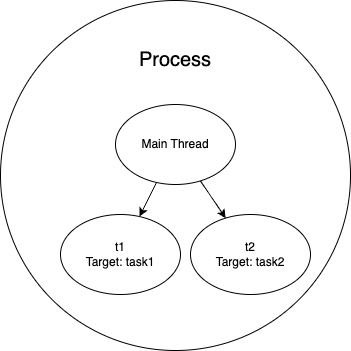
\includegraphics[width=0.5\textwidth]{/Users/khawaritzmi/Unhas/os_report_mid2024/b_class/asset/example.png}  % Sesuaikan nama file dan ukurannya
    \caption{Ini adalah gambar contoh dari multithreading.}
    \label{fig:contoh_gambar}
\end{figure}

Seperti yang terlihat pada Gambar \ref{fig:contoh_gambar}, inilah cara menambahkan gambar dengan keterangan.

\subsection{File Systems}
\subsubsection{Access Methods}
Metode akses file mengacu pada cara file dibaca, ditulis, atau dimodifikasi dalam sistem file. Ada beberapa metode akses yang digunakan dalam sistem file untuk memungkinkan aplikasi atau pengguna mengambil dan memanipulasi data dalam file. Berikut adalah penjelasan rinci mengenai metode akses file yang umum digunakan:

\begin{enumerate}
    \item Akses Berurutan \textit{(Sequential Access)}
    
    \textit{Sequential Access} adalah metode akses file di mana data diakses secara berurutan, dari awal hingga akhir. Ini mirip dengan cara kita membaca sebuah buku, satu halaman per satu secara berurutan.

    {Deskripsi:}
    \begin{itemize}
        \item Dalam metode akses ini, file diakses dalam urutan linier tertentu, dari awal hingga akhir. Data dibaca atau ditulis secara berurutan, mirip dengan cara kerja kaset magnetik, di mana untuk membaca bagian tertentu dari data, seluruh file harus dilalui dari awal hingga posisi data tersebut ditemukan.
        \item Ini adalah metode akses yang paling sederhana dan sering digunakan untuk aplikasi yang memerlukan pemrosesan data dalam urutan tetap.
    \end{itemize}

    \begin{figure}[h]
        \centering
        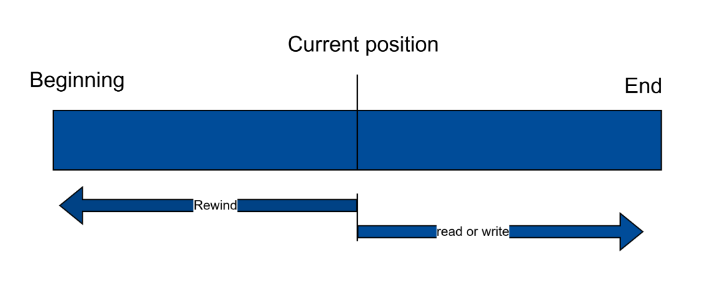
\includegraphics[width=0.5\linewidth]{assets/Screenshot 2024-09-30 184303.png}
        \caption{Metode Akses Berurutan}
        \label{fig:sequential-access}
    \end{figure}

    {Deskripsi gambar:}
     \begin{itemize}
        \item Current Position: Menunjukkan posisi saat ini dalam file di mana data akan dibaca atau ditulis. Posisi ini akan bergerak maju setiap kali data dibaca atau ditulis.

        \item \textit{Rewind}: Jika ingin kembali ke bagian sebelumnya dari file, perlu dilakukan \textit{"rewind"} atau mundur dari posisi saat ini untuk kembali ke posisi sebelumnya (atau bahkan ke awal file).

        \item \textit{Read and write}: File dibaca atau ditulis secara linier dari posisi saat ini menuju ke akhir file. Data diproses satu per satu dalam urutan dari kiri ke kanan

    \end{itemize}

    {Kasus penggunaan:}
     \begin{itemize}
        \item Arsip

        \item Media file

        \item Sistem \textit{backup}: Penyimpanan data yang diakses atau dipulihkan secara berurutan.

    \end{itemize}

    {Kelebihan:}
     \begin{itemize}
        \item Sederhana: Metode ini mudah diimplementasikan dan ideal untuk penggunaan di mana urutan data penting.


        \item Kinerja: Dapat memberikan kinerja yang baik untuk aplikasi yang membaca atau menulis seluruh file dari awal hingga akhir.
    \end{itemize}

    {Kekurangan:}
     \begin{itemize}
        \item Tidak Fleksibel: Untuk mengakses data di tengah file, seluruh bagian sebelumnya harus dilewati, membuat akses menjadi lambat untuk file besar.

        \item Tidak efisien: Untuk aplikasi yang memerlukan pengambilan data secara acak, metode ini tidak efisien.

    \end{itemize}

    
\item  Akses Langsung atau Acak \textit{(Direct or Random Access)}

Direct access adalah metode akses file di mana kita dapat langsung mengakses data pada posisi tertentu tanpa harus membaca seluruh file dari awal. Ini memungkinkan akses yang lebih cepat dan efisien.

    {Deskripsi:}
    \begin{itemize}
        \item Dalam metode akses langsung, setiap bagian file dapat diakses secara langsung tanpa perlu membaca data secara berurutan. Sistem dapat melompat ke posisi mana pun dalam file, memungkinkan pengguna untuk membaca atau menulis data di bagian tertentu tanpa harus memproses seluruh file.

        \item Akses langsung dimungkinkan karena perangkat penyimpanan modern seperti hard disk drive (HDD) dan solid-state drive (SSD) mendukung lompatan ke lokasi byte atau blok tertentu.
    \end{itemize}

    \begin{figure}[h]
        \centering
        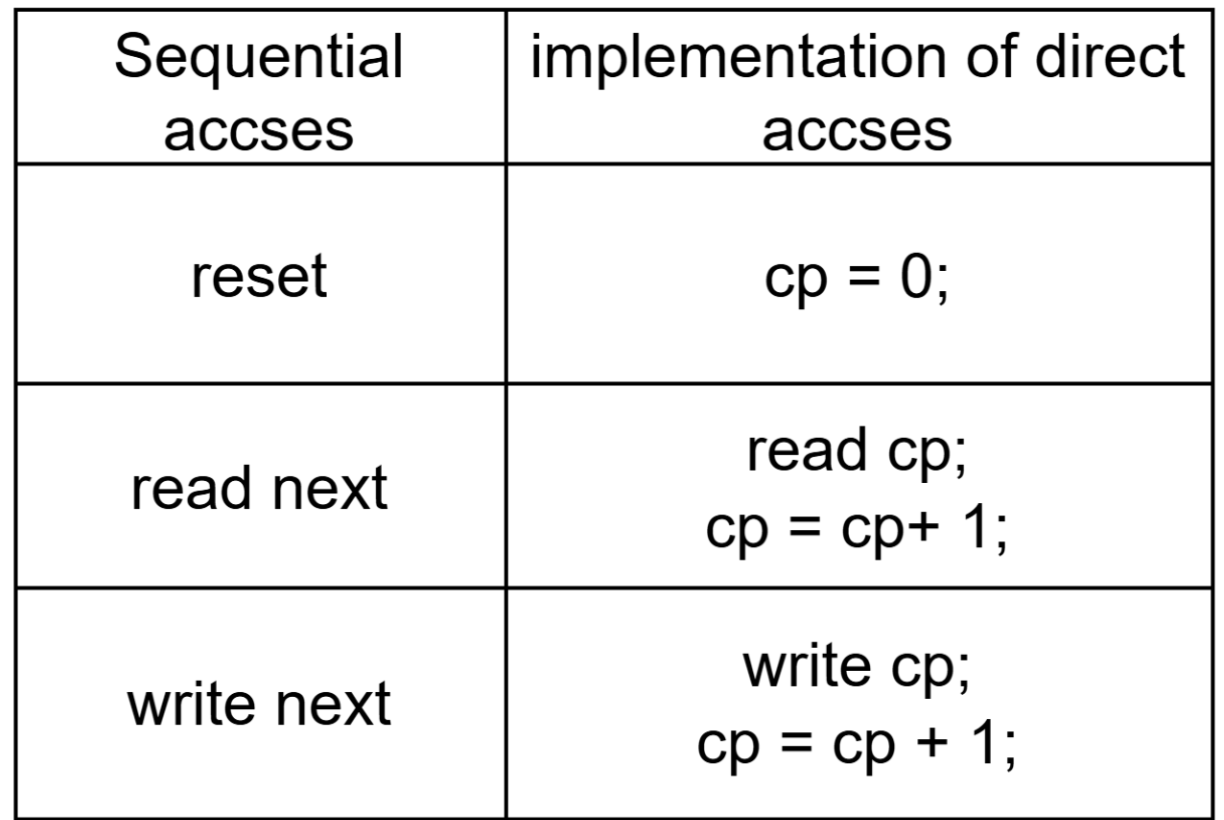
\includegraphics[width=0.5\linewidth]{assets/p2.png}
        \caption{Metode Akses Langsung}
        \label{fig:sequential-access}
    \end{figure}

    {Deskripsi gambar:}
     \begin{itemize}
        \item \textit{Reset}
        \begin{itemize}
            \item \textit{Sequential Access}: Reset berarti mengembalikan posisi file ke awal, agar dapat diakses dari posisi pertama.
            
            \item \textit{Direct Access}: Pada akses langsung, ini diimplementasikan dengan mengatur variabel cp (current position) menjadi 0 (), yang berarti mengarahkan penunjuk file ke posisi pertama
        
        \end{itemize}

        \item \textit{Read Next}:
        \begin{itemize}
        \item \textit{Sequential Access}: Membaca file berikutnya berarti membaca data secara berurutan, satu per satu.

        \item \textit{Direct Access}: Dalam akses langsung, membaca data dilakukan dari posisi yang ditunjukkan oleh cp (). Setelah membaca data, posisi file kemudian ditingkatkan dengan 1 (), sehingga penunjuk siap membaca data berikutnya
        
        \end{itemize}

        \item \textit{Write Next}: File dibaca atau ditulis secara linier dari posisi saat ini menuju ke akhir file. Data diproses satu per satu dalam urutan dari kiri ke kanan
         \begin{itemize}
        \item \textit{Sequential Access} : Menulis data berikutnya dilakukan secara berurutan, setelah data yang sudah ada.

            
        \item \textit{Direct Access}: Dalam akses langsung, menulis dilakukan pada posisi cp saat ini (). Setelah menulis data, posisi penunjuk juga ditingkatkan dengan 1 (), sehingga siap untuk menulis data selanjutnya.
        
        \end{itemize}

    \end{itemize}

    {Kasus penggunaan:}
     \begin{itemize}
        \item Basis data (Database): Akses langsung memungkinkan pengambilan catatan individu dalam database tanpa perlu membaca seluruh file.

        \item File indeks: Dalam file indeks, posisi tertentu di dalam file dapat diakses dengan cepat berdasarkan nilai kunci.

        \item File konfigurasi: File yang memerlukan modifikasi pada bagian tertentu tanpa mengubah keseluruhan isi file.


    \end{itemize}

    {Kelebihan:}
     \begin{itemize}
        \item Efisiensi: Metode ini sangat efisien untuk aplikasi yang memerlukan akses cepat ke bagian tertentu dari file tanpa harus membaca keseluruhan file.

        \item Fleksibilitas: Data dapat dimodifikasi, ditambah, atau dihapus pada bagian mana pun dalam file
    \end{itemize}

    {Kekurangan:}
     \begin{itemize}
        \item Lebih rumit: Implementasi akses langsung membutuhkan manajemen lebih kompleks untuk melacak lokasi fisik data pada media penyimpanan.

        \item Overhead: Mengelola dan memelihara indeks atau metadata untuk mendukung akses langsung bisa menambah overhead.

    \end{itemize}



\item  Akses Terindex \textit{(Indexes Access)}

    {Deskripsi:}
    \begin{itemize}
        \item Akses terindeks menggunakan indeks yang mengaitkan nilai kunci dengan lokasi blok data di dalam file. Indeks berfungsi seperti daftar isi yang memungkinkan sistem untuk menemukan lokasi data tanpa harus menelusuri seluruh file.

        \item Setiap entri dalam indeks berisi kunci pencarian dan pointer ke lokasi data yang sesuai di file.
    \end{itemize}

    {Kasus penggunaan:}
     \begin{itemize}
        \item Sistem basis data: Pengindeksan sering digunakan dalam database untuk mempercepat pencarian data berdasarkan kunci unik (misalnya, nomor ID atau nama).

        \item File besar: Dalam file yang sangat besar atau file yang berisi jutaan catatan, indeks memungkinkan pencarian data yang cepat.

    \end{itemize}

    {Kelebihan:}
     \begin{itemize}
        \item Pencarian cepat: Akses ke data sangat cepat, bahkan dalam file yang sangat besar, karena pencarian langsung dilakukan melalui indeks tanpa membaca file secara keseluruhan.

        \item Skalabilitas: Dapat diimplementasikan dalam sistem besar dengan banyak data.

    \end{itemize}

    {Kekurangan:}
     \begin{itemize}
        \item Overhead penyimpanan: Indeks memerlukan ruang tambahan untuk menyimpan informasi indeks.
        
        \item Overhead pemeliharaan: Indeks harus diperbarui setiap kali ada perubahan pada file (misalnya, penambahan atau penghapusan data), yang dapat menyebabkan peningkatan beban kerja.

    \end{itemize}

\end{enumerate}


\subsection{Deadlock Introduction and Prevention}
Explores the concept of deadlocks and methods for preventing them:
\begin{itemize}
    \item Deadlock conditions
    \item Deadlock prevention techniques
\end{itemize}

\subsection{User Interface Management}
This section discusses the role of the operating system in managing the user interface. Topics covered include:
\begin{itemize}
    \item Graphical User Interface (GUI)
    \item Command-Line Interface (CLI)
    \item Interaction between the user and the operating system
\end{itemize}

\subsection{Virtualization in Operating Systems}
Virtualization allows multiple operating systems to run concurrently on a single physical machine. This section explores:
\begin{itemize}
    \item Concept of virtualization
    \item Hypervisors and their types
    \item Benefits of virtualization in modern computing
\end{itemize}

\section{Assignments and Practical Work}
\subsection{Assignment 1: Process Scheduling}
Students were tasked with implementing various process scheduling algorithms (e.g., FCFS, SJN, and RR) and comparing their performance under different conditions.
\subsubsection{Group 1}
\begin{python}
    class Process:
    def __init__(self, pid, arrival_time, burst_time):
        self.pid = pid
        self.arrival_time = arrival_time
        self.burst_time = burst_time
        self.completion_time = 0
        self.turnaround_time = 0
        self.waiting_time = 0
\end{python}

\begin{table}[htbp] % Optional: For floating position
    \centering
    \begin{tabular}{|c|c|c|} % Defines number of columns and alignment (c = center, l = left, r = right). '|' creates vertical lines.
    \hline
    Header 1 & Header 2 & Header 3 \\ % Column headers
    \hline
    Row 1, Column 1 & Row 1, Column 2 & Row 1, Column 3 \\ % First row of data
    \hline
    Row 2, Column 1 & Row 2, Column 2 & Row 2, Column 3 \\ % Second row of data
    \hline
    \end{tabular}
    \caption{Your table caption} % Optional: For adding a caption
    \label{tab:your_label} % Optional: For cross-referencing the table
\end{table}

\subsection{Assignment 2: Deadlock Handling}
In this assignment, students were asked to simulate different deadlock scenarios and explore various prevention methods.

\subsection{Assignment 3: Multithreading and Amdahl's Law}
This assignment involved designing a multithreading scenario to solve a computationally intensive problem. Students then applied **Amdahl's Law** to calculate the theoretical speedup of the program as the number of threads increased.

\subsection{Assignment 4: Simple Command-Line Interface (CLI) for User Interface Management}
Students were tasked with creating a simple **CLI** for user interface management. The CLI should support basic commands such as file manipulation (creating, listing, and deleting files), process management, and system status reporting.
\subsubsection{Group 8}
Buatlah sebuah program Python yang menyediakan antarmuka pengguna berbasis teks (CLI) untuk manajemen file dan proses. Buatlah beberapa \textit{function} dalam python
\begin{itemize}
    \item Membuat file baru dengan nama yang ditentukan.
    \item Menampilkan daftar file yang ada di direktori saat ini.
    \item Menghapus file dengan nama yang ditentukan
    \item Menampilkan daftar proses yang sedang berjalan di sistem.
    \item Menampilkan status sistem, termasuk penggunaan memori dan ruang disk.
    \item Keluar dari program.
\end{itemize}
\begin{python}
import os
import psutil

# Fungsi untuk membuat file baru
def create_file(file_name):
    try:
        # Membuka file dalam mode tulis ('w'), akan membuat file baru jika tidak ada
        with open(file_name, 'w') as f:
            f.write("")  # Membuat file kosong
        print(f"File '{file_name}' berhasil dibuat.")
    except Exception as e:
        print(f"Error saat membuat file: {e}")

# Fungsi untuk menampilkan daftar file di direktori saat ini
def list_files():
    try:
        # Mengambil daftar file di direktori saat ini
        files = os.listdir(".")
        if files:
            print("Daftar file:")
            for file in files:
                print(f" - {file}")  # Menampilkan nama file
        else:
            print("Tidak ada file di direktori saat ini.")
    except Exception as e:
        print(f"Error saat menampilkan file: {e}")

# Fungsi untuk menghapus file
def delete_file(file_name):
    try:
        # Mengecek apakah file ada sebelum menghapus
        if os.path.exists(file_name):
            os.remove(file_name)  # Menghapus file
            print(f"File '{file_name}' berhasil dihapus.")
        else:
            print(f"File '{file_name}' tidak ditemukan.")
    except Exception as e:
        print(f"Error saat menghapus file: {e}")

# Fungsi untuk menampilkan proses yang berjalan
def list_processes():
    try:
        print("Daftar proses yang sedang berjalan:")
        # Iterasi melalui proses yang sedang berjalan
        for proc in psutil.process_iter(['pid', 'name']):
            print(f"PID: {proc.info['pid']} - Nama Proses: {proc.info['name']}")
    except Exception as e:
        print(f"Error saat menampilkan proses: {e}")

# Fungsi untuk menampilkan status sistem (memori dan disk)
def system_status():
    try:
        # Mengambil informasi memori dan disk
        mem = psutil.virtual_memory()
        disk = psutil.disk_usage('/')
        print("Status Sistem:")
        print(f"Memori yang Digunakan: {mem.percent}%")
        print(f"Ruang Disk yang Digunakan: {disk.percent}%")
    except Exception as e:
        print(f"Error saat menampilkan status sistem: {e}")

# Fungsi untuk menjalankan perintah CLI
def run_cli():
    print("Simple CLI untuk Manajemen Antarmuka Pengguna")
    print("Perintah yang tersedia: create <file_name>, list, delete <file_name>, process, status, exit")

    while True:
        # Menerima input perintah dari pengguna
        command = input("Masukkan perintah: ").split()

        # Jika tidak ada perintah yang dimasukkan, lanjutkan ke input berikutnya
        if len(command) == 0:
            continue

        cmd = command[0]  # Mengambil perintah pertama

        if cmd == "create":
            # Memastikan nama file diberikan
            if len(command) > 1:
                create_file(command[1])
            else:
                print("Nama file tidak diberikan.")

        elif cmd == "list":
            list_files()  # Menampilkan daftar file

        elif cmd == "delete":
            # Memastikan nama file diberikan
            if len(command) > 1:
                delete_file(command[1])
            else:
                print("Nama file tidak diberikan.")

        elif cmd == "process":
            list_processes()  # Menampilkan daftar proses yang sedang berjalan

        elif cmd == "status":
            system_status()  # Menampilkan status sistem

        elif cmd == "exit":
            print("Keluar dari CLI.")  # Menyatakan keluar dari CLI
            break

        else:
            print(f"Perintah '{cmd}' tidak dikenal.")  # Menyatakan perintah tidak dikenal

# Jalankan CLI
if __name__ == "__main__":
    run_cli()

\end{python}

\subsection{Assignment 5: File System Access}
In this assignment, students implemented file system access routines, includ
ing: 
\begin{itemize}
    \item File creation and deletion
    \item Reading from and writing to files
    \item Navigating directories and managing file permissions
\end{itemize}
\subsubsection{Group 8}
Buatlah program Python sebagai sistem manajamen file yang sederhana serta lakukan beberapa memiliki fitur-fitur seperti ini:
\begin{itemize}
    \item Membuat File: Program harus dapat membuat file baru dengan nama yang diberikan oleh pengguna.
    \item Menghapus File: Program harus dapat menghapus file yang sudah ada berdasarkan nama file yang diberikan oleh pengguna.
    \item Menulis ke File: Program harus dapat menulis data ke file yang ditentukan, dengan opsi untuk menggunakan mode
    \textit{append} (menambah di akhir) atau \textit{overwrite} (mengganti isi).
    \item Berpindah Direktori: Program harus dapat berpindah ke direktori yang ditentukan oleh pengguna.
    \item Cek Izin Akses File: Program harus dapat memeriksa dan menampilkan izin akses dari file yang diberikan.
    \item Keluar dari Program: Program harus dapat berhenti berjalan ketika pengguna memilih untuk keluar.
\end{itemize}
Program harus terus meminta perintah dari pengguna hingga pengguna memilih untuk keluar, dan memberikan umpan balik sesuai dengan hasil setiap operasi. Gunakan \textit{try} dan \textit{except} untuk menangani kemungkinan kesalahan, seperti file yang tidak ditemukan atau direktori yang tidak ada.
\begin{python}
import os

# Fungsi untuk membuat file baru
def create_file(nama_file):
    try:
        with open(nama_file, 'x') as f:
            print(f"File '{nama_file}' berhasil dibuat.")
    except FileExistsError:
        print(f"File '{nama_file}' sudah ada.")

# Fungsi untuk menghapus file
def delete_file(nama_file):
    try:
        os.remove(nama_file)
        print(f"File '{nama_file}' berhasil dihapus.")
    except FileNotFoundError:
        print(f"File '{nama_file}' tidak ditemukan.")

# Fungsi untuk membaca file
def read_file(nama_file):
    try:
        with open(nama_file, 'r') as f:
            print(f"Isi file '{nama_file}':")
            print(f.read())
    except FileNotFoundError:
        print(f"File '{nama_file}' tidak ditemukan.")

# Fungsi untuk menulis ke file
def write_file(nama_file, data, mode='a'):
    try:
        with open(nama_file, mode) as f:
            f.write(data + "\n")
            print(f"Data berhasil ditulis ke file '{nama_file}' dalam mode '{mode}'.")
    except Exception as e:
        print(f"Terjadi kesalahan saat menulis ke file: {e}")

# Fungsi untuk berpindah direktori
def change_directory(path):
    try:
        os.chdir(path)
        print(f"Berhasil berpindah ke direktori: {os.getcwd()}")
    except FileNotFoundError:
        print(f"Direktori '{path}' tidak ditemukan.")
    except Exception as e:
        print(f"Terjadi kesalahan: {e}")

# Fungsi untuk memeriksa izin akses file
def check_permissions(nama_file):
    try:
        permissions = os.stat(nama_file)
        print(f"Izin akses untuk file '{nama_file}':")
        print(f"Readable: {'Ya' if os.access(nama_file, os.R_OK) else 'Tidak'}")
        print(f"Writable: {'Ya' if os.access(nama_file, os.W_OK) else 'Tidak'}")
        print(f"Executable: {'Ya' if os.access(nama_file, os.X_OK) else 'Tidak'}")
    except FileNotFoundError:
        print(f"File '{nama_file}' tidak ditemukan.")

# Fungsi utama untuk menjalankan CLI
def main():
    while True:
        print("\nAkses Sistem Berkas CLI")
        print("1. create <nama_file> : Membuat file baru")
        print("2. delete <nama_file> : Menghapus file")
        print("3. read <nama_file>   : Membaca isi file")
        print("4. write <nama_file> <mode> : Menulis ke file (mode 'a' untuk append, 'w' untuk overwrite)")
        print("5. cd <path>          : Berpindah direktori")
        print("6. permissions <nama_file> : Cek izin akses file")
        print("7. exit               : Keluar dari program")

        user_input = input("\nMasukkan perintah: ").split()

        if len(user_input) == 0:
            print("Perintah tidak valid. Silakan coba lagi.")
            continue

        command = user_input[0]

        if command == 'create' and len(user_input) == 2:
            create_file(user_input[1])

        elif command == 'delete' and len(user_input) == 2:
            delete_file(user_input[1])

        elif command == 'read' and len(user_input) == 2:
            read_file(user_input[1])

        elif command == 'write' and len(user_input) >= 3:
            nama_file = user_input[1]
            mode = user_input[2]
            data = input("Masukkan data untuk ditulis: ")
            write_file(nama_file, data, mode)

        elif command == 'cd' and len(user_input) == 2:
            change_directory(user_input[1])

        elif command == 'permissions' and len(user_input) == 2:
            check_permissions(user_input[1])

        elif command == 'exit':
            print("Keluar dari program.")
            break

        else:
            print("Perintah tidak valid. Silakan coba lagi.")

# Menjalankan program
if __name__ == "__main__":
    main()

\end{python}

\section{Conclusion}
The first half of the course introduced core operating system concepts, including process management, scheduling, multithreading, and file system access. These topics provided a foundation for more advanced topics to be covered in the second half of the course.

\end{document}